\documentclass[12pt,a4paper]{article}
\usepackage[top=1in,bottom=1in,left=1.25in,right=1.25in]{geometry}
\usepackage{times}
\usepackage{setspace}
\usepackage{graphicx}
\usepackage{amsmath}
\usepackage{booktabs}
\usepackage{hyperref}
\usepackage{titlesec}
\usepackage{fancyhdr}
\usepackage{xcolor}
\usepackage{parskip}
\usepackage{tikz}
\usetikzlibrary{positioning, arrows.meta, backgrounds, fit, shapes.geometric}

\setstretch{1.3}

\hypersetup{
    colorlinks=true,
    linkcolor=black,
    urlcolor=blue
}

\titleformat{\section}{\large\bfseries}{\thesection.}{0.6em}{}
\titleformat{\subsection}{\normalsize\bfseries}{\thesubsection.}{0.5em}{}
\titlespacing{\section}{0pt}{14pt}{6pt}
\titlespacing{\subsection}{0pt}{10pt}{4pt}

\pagestyle{fancy}
\fancyhf{}
\lhead{\small BCSE329L -- Blockchain and Distributed Ledger Technology}
\rhead{\small Digital Assignment}
\cfoot{\thepage}
\renewcommand{\headrulewidth}{0.4pt}

\begin{document}

% ─── Title Page ───────────────────────────────────────────────────
\begin{titlepage}
\centering
\vspace*{1.5cm}
{\Large\bfseries Vellore Institute of Technology, Vellore}\\[0.4cm]
{\normalsize School of Computer Science and Engineering}\\[0.2cm]
{\normalsize BCSE329L -- Blockchain and Distributed Ledger Technology}\\
\vspace{0.3cm}
\hrule height 0.8pt
\vspace{0.8cm}

{\LARGE\bfseries Digital Assignment\\[0.3cm]
Course Project \& Hyperledger Architectures}

\vspace{1.2cm}
\begin{tabular}{ll}
\textbf{Submitted by:}  & Mihir Dixit \\
\textbf{Reg. No.:}      & 23BKT0073 \\
\textbf{Programme:}     & B.Tech -- Computer Science and Engineering \\
\textbf{Subject Code:}  & BCSE329L \\
\textbf{Faculty:}       & Dr. Sivaranjani A \\
\end{tabular}

\vspace*{\fill}
\hrule height 0.8pt
\end{titlepage}

\tableofcontents
\newpage

% ═══════════════════════════════════════════════════════════════════
\section{1. Hyperledger Fabric Using Docker}
% ═══════════════════════════════════════════════════════════════════

A consortium of two organizations intending to trace assets can leverage Hyperledger Fabric due to its permissioned, channel-based design. Deploying this network locally using Docker involves defining containers for each architectural component and linking them via a virtual Docker network.

\begin{figure}[!htbp]
\centering
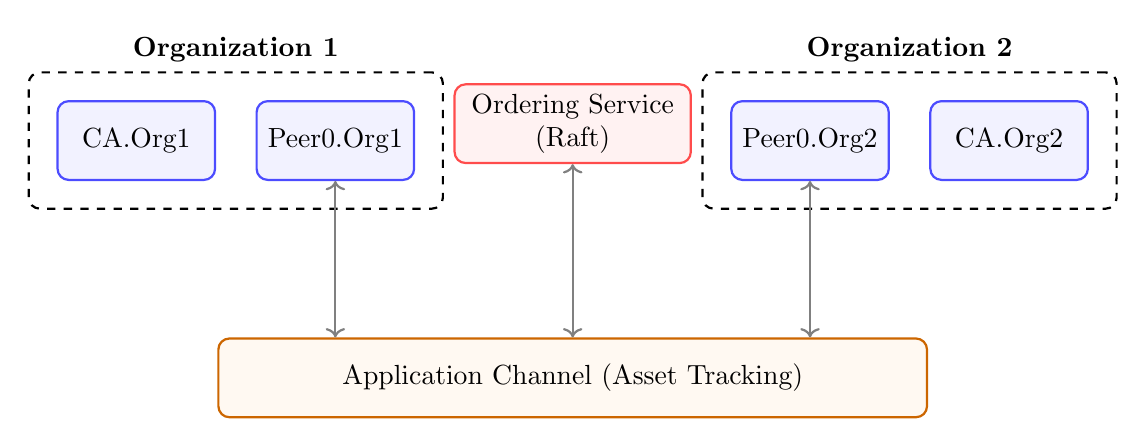
\begin{tikzpicture}[
    node distance=1.5cm,
    orgbox/.style={draw=black, dashed, thick, rounded corners, inner sep=10pt},
    nodeitem/.style={draw=blue!70, fill=blue!5, thick, rectangle, rounded corners, align=center, minimum width=2cm, minimum height=1cm},
    orderer/.style={draw=red!70, fill=red!5, thick, rectangle, rounded corners, align=center, minimum width=3cm, minimum height=1cm},
    channel/.style={draw=orange!80!black, fill=orange!5, thick, rectangle, rounded corners, align=center, minimum width=9cm, minimum height=1cm},
    arrow/.style={-{Stealth[length=2mm]}, thick, gray}
]

% Channel at the bottom
\node[channel] (channel) {Application Channel (Asset Tracking)};

% Org1
\node[nodeitem, above=2.5cm of channel.west, xshift=1.5cm] (peer1) {Peer0.Org1};
\node[nodeitem, left=0.5cm of peer1] (ca1) {CA.Org1};
\begin{scope}[on background layer]
    \node[orgbox, fit=(peer1) (ca1), label=above:\textbf{Organization 1}] (org1) {};
\end{scope}

% Org2
\node[nodeitem, above=2.5cm of channel.east, xshift=-1.5cm] (peer2) {Peer0.Org2};
\node[nodeitem, right=0.5cm of peer2] (ca2) {CA.Org2};
\begin{scope}[on background layer]
    \node[orgbox, fit=(peer2) (ca2), label=above:\textbf{Organization 2}] (org2) {};
\end{scope}

% Orderer
\node[orderer, above=2.2cm of channel] (orderer) {Ordering Service \\ (Raft)};

% Connections
\draw[arrow, <->] (peer1.south) -- (channel.north -| peer1.south);
\draw[arrow, <->] (peer2.south) -- (channel.north -| peer2.south);
\draw[arrow, <->] (orderer.south) -- (channel.north -| orderer.south);

\end{tikzpicture}
\caption{Hyperledger Fabric Network Architecture for Asset Tracking}
\end{figure}

\subsection{Network Architecture and Roles}

\begin{itemize}
    \item \textbf{Organizations (Org1, Org2):} Represent the participants in the consortium. Each has its own distinct membership and policies.
    \item \textbf{Certificate Authority (CA):} Each organization uses a Fabric CA to issue X.509 identity certificates for administrators, peer nodes, and client applications.
    \item \textbf{Ordering Service:} A cluster of nodes (typically Raft) that receives endorsed transactions, orders them chronologically, and cuts them into blocks. It ensures global state consistency but does not execute smart contracts.
    \item \textbf{Peers:} Nodes belonging to Org1 and Org2 that maintain a copy of the ledger and run the chaincode containers to simulate transactions.
    \item \textbf{Channels:} A private communication subnet. Only peers that join the asset-tracking channel possess the ledger and chaincode relevant to those assets.
    \item \textbf{Ledger:} Consists of a blockchain holding transaction records and a world state database (e.g., CouchDB) storing current asset states.
    \item \textbf{Chaincode:} The smart contract containing the programmatic rules for asset creation, transfer, and query functionality.
\end{itemize}

\subsection{Deployment Procedure}

\textbf{1. Generate Cryptographic Materials:}\\
Define the network topology in a configuration file and execute \texttt{cryptogen} to generate the necessary private keys and certificates for Org1, Org2, and the Orderer.

\textbf{2. Create Genesis Block and Channel Transactions:}\\
Use the \texttt{configtxgen} tool to read \texttt{configtx.yaml} and produce the genesis block for the ordering service. Generate an envelope transaction for creating the application channel.

\textbf{3. Deploy Docker Containers:}\\
Execute \texttt{docker-compose up -d} using a \texttt{docker-compose.yaml} file that defines images, volume mounts, and environment variables for the CA, Orderer, Peer, and CLI containers.

\textbf{4. Channel Creation and Joining:}\\
From the CLI container, run \texttt{peer channel create} using the generated envelope transaction. Then, command peer nodes from Org1 and Org2 to execute \texttt{peer channel join} to attach themselves to the channel lattice.

\textbf{5. Chaincode Deployment:}\\
Package the chaincode using \texttt{peer lifecycle chaincode package}. Install it on the peers, approve the chaincode definition on behalf of both organizations, and finally commit the definition to the channel.

\textbf{6. Perform Transactions:}\\
Utilize \texttt{peer chaincode invoke} to write new asset data to the ledger and \texttt{peer chaincode query} to retrieve asset states via the consensus pathway.

% ═══════════════════════════════════════════════════════════════════
\section{2. Hyperledger Fabric Blockchain Service on AWS Cloud}
% ═══════════════════════════════════════════════════════════════════

Migrating the Hyperledger Fabric asset-tracking network to a cloud environment ensures production-grade resilience. Over Amazon Web Services (AWS), the architecture leverages native infrastructure to isolate and monitor the blockchain nodes effectively.

\subsection{AWS Architecture Design}

\begin{itemize}
    \item \textbf{Amazon VPC (Virtual Private Cloud):} Establishes an isolated network boundary.
    \item \textbf{Subnets:} Public subnets hold NAT Gateways and Bastion Hosts for secure administrative access. Private subnets host the EC2 instances running orderer and peer nodes, hiding them from the public internet.
    \item \textbf{Amazon EC2:} Virtual server instances operating as Docker hosts for the Fabric containers. Separate instances should ideally be allocated for Org1 peers, Org2 peers, and the Ordering nodes to avoid contention.
    \item \textbf{Security Groups:} Serve as stateful firewalls. Rules allow ingress on port 7051 (Peer) and 7050 (Orderer) only from within the internal VPC CIDR block.
    \item \textbf{Amazon EBS (Elastic Block Store):} Configured as persistent Docker volumes mapped directly to the Fabric peer ledgers. If an EC2 instance reboots, the world state remains intact on EBS.
    \item \textbf{IAM (Identity and Access Management):} Applies the principle of least privilege, allowing developers partial EC2 access while blocking deletion rights over the EBS volumes.
    \item \textbf{Amazon CloudWatch:} Docker logging drivers on EC2 route container logs (e.g., chaincode output or peer gossip logs) into CloudWatch for aggregated monitoring and alerting.
\end{itemize}

\subsection{Comparison: Local Docker vs. AWS Deployment}

\begin{itemize}
    \item \textbf{Security:} Local deployment uses only namespace-level isolation via Docker. AWS provides deep defense layers including VPC gating, Security Groups, and IAM restrictions, severely limiting attack vectors.
    \item \textbf{Scalability:} Expanding a local network is hardware-constrained. In AWS, upgrading EC2 hardware or launching new peer nodes across different Availability Zones (AZs) is instantaneous.
    \item \textbf{Availability:} Local configurations create a massive Single Point of Failure (SPOF) at the host physical machine level. AWS supports Multi-AZ deployments, ensuring ledger access continues even if an entire AWS data center goes offline.
    \item \textbf{Cost:} A local environment costs nearly nothing for testing but requires massive upfront capital expenditure (CapEx) to scale servers for production. AWS relies on an Operational Expenditure (OpEx) model consisting of hourly fees for compute and storage.
    \item \textbf{Management:} Monitoring a local network requires manual ELK stack or Prometheus configurations. AWS handles management autonomously through CloudWatch and Systems Manager.
\end{itemize}

% ═══════════════════════════════════════════════════════════════════
\section{3. Course Project: First Functional Module Implementation}
% ═══════════════════════════════════════════════════════════════════

\textbf{Project Name:} zk-dPKI (Decentralized Public Key Infrastructure) \\
\textbf{Focus Area:} Setup and initial implementation of the first functional module.

\subsection{Module Identity and Overview}
\textbf{What the module represents:} The implemented module constitutes the \textit{Consensus Engine and Base Ledger Certification Layer} of the zk-dPKI system. This represents approximately 35\% of the final project scope.

\textbf{Purpose and functionality:} Its purpose is to physically replace the standard Certificate Authority (CA) with a distributed network paradigm. It achieves this by taking identity inputs, simulating Byzantine Fault Tolerant (BFT) negotiation over blocks, and securely issuing Decentralized Identifiers (DIDs) linked exclusively to on-chain hash commitments.

\textbf{Contribution to the overall project:} The entire zero-knowledge privacy aspect of the project relies on this ledger for trust. Without a functional decentralized root-of-trust recording immutable certificate commitments, there is no verifiable reference point against which ZK proofs can be evaluated.

\subsection{Code Mechanics and Components}
\textbf{How the submitted code works:} 
The architecture operates efficiently within a dual-script controller design:
\begin{itemize}
    \item \texttt{network.js}: Controls the simulated blockchain state. It maintains the registry of peer nodes and defines \texttt{Network.issueCertificate()}, which packages the transaction. It houses \texttt{runConsensusRound()} to enforce BFT logic (simulating Prevote and Precommit stages).
    \item \texttt{app.js}: Bridges ledger logic to the Document Object Model (DOM). It updates the live block feed and visually transitions peer node cards from 'Idle' to 'Voting' to 'Agreed' based on consensus callbacks.
    \item \texttt{style.css / index.html}: Deliver a custom minimalist visual framework avoiding pre-built templates, ensuring direct feedback on the blockchain's block height and metrics.
\end{itemize}

\subsection{Technologies and Blockchains Used}
\textbf{Technologies utilized:} Vanilla JavaScript (ES6+), HTML5 Canvas for real-time network topology rendering, CSS3, and standard Web Crypto APIs for hashing operations. 

\textbf{Blockchain incorporation specifics:} The project models a permissioned smart contract environment running an IBFT-2/HotStuff consensus. Specifically, it executes the operations of a \texttt{DAOGovernor.sol} smart contract entirely via simulated JS functions. The CA's central database is completely removed; instead, the certificate commitment merges into a ledger block, ensuring immutability through hash linking.

\subsection{Data Inputs and Setup Instructions}
\textbf{Data inputs used:} The module accepts identity attributes during the issuance test phase. Inputs primarily consist of Common Name (e.g., Alice Sharma), Organization (e.g., QuantumTech), RBAC Role parameters, and MAC clearance designations.

\textbf{Initial setup required:}
The module relies on modern cryptography APIs that modern web browsers strict-block under the \texttt{file://} protocol. Running it locally requires a local HTTP server.
\begin{enumerate}
    \item Ensure Python 3 is installed.
    \item Navigate to the project root directory containing \texttt{index.html}.
    \item Execute standard web hosting command: \texttt{python -m http.server 3000}
    \item Open a web browser and connect to \texttt{http://localhost:3000}
\end{enumerate}

\subsection{Working Status and Demonstration}

The module successfully achieves issuance and simulates block generation. 
The following screenshots provide a demonstration of the live consensus network, the issuance outcome, and the Merkle tree functionality operations.

\begin{figure}[!htbp]
    \centering
    \vspace{8cm} % Paste your Part 1 image here
    \caption{Working Status Demonstration (Part 1)}
\end{figure}

\begin{figure}[!htbp]
    \centering
    \vspace{8cm} % Paste your Part 2 image here
    \caption{Working Status Demonstration (Part 2)}
\end{figure}

\begin{figure}[!htbp]
    \centering
    \vspace{8cm} % Paste your Part 3 image here
    \caption{Working Status Demonstration (Part 3)}
\end{figure}

\begin{figure}[!htbp]
    \centering
    \vspace{8cm} % Paste your Part 4 image here
    \caption{Working Status Demonstration (Part 4)}
\end{figure}

\begin{figure}[!htbp]
    \centering
    \vspace{8cm} % Paste your Part 5 image here
    \caption{Working Status Demonstration (Part 5)}
\end{figure}

\begin{figure}[!htbp]
    \centering
    \vspace{8cm} % Paste your Part 6 image here
    \caption{Working Status Demonstration (Part 6)}
\end{figure}

\end{document}
